O produto foi idealizado como sendo um sistema capaz de integrar vários balões à área a ser monitorada, que será o estacionamento da faculdade UnB Gama.

Foram definidos cinco pontos estratégicos de localização dos balões cativos, que podem ser vistos na figura \ref{img:localizacao-baloes}, para que não possuam pontos cegos.


\begin{figure}[H]
	\centering
	\caption{Localização dos balões no campus FGA}
	\includegraphics[width=0.7\textwidth]{figuras/localizacao-baloes}
	\label{img:localizacao-baloes}
\end{figure}


Para o melhor entendimento do funcionamento geral do Sistema Unificado de Monitoramento pelo leitor, foi feito, com o uso do programa \emph{CoreIDRAW X7}, uma ilustração simplificada (figura \ref{img:ilus-fun-sum}) da disposição de alguns balões, estes presos no terraço do prédio da faculdade, e a estação de solo, localizada ao lado do prédio. Todos os elementos do projeto foram enumerados  para que, em seguida, o leitor possa acompanhar o funcionamento geral e a disposição da solução específica no presente relatório.

\begin{figure}[H]
\centering
\caption{Ilustração do funcionamento do SUM}
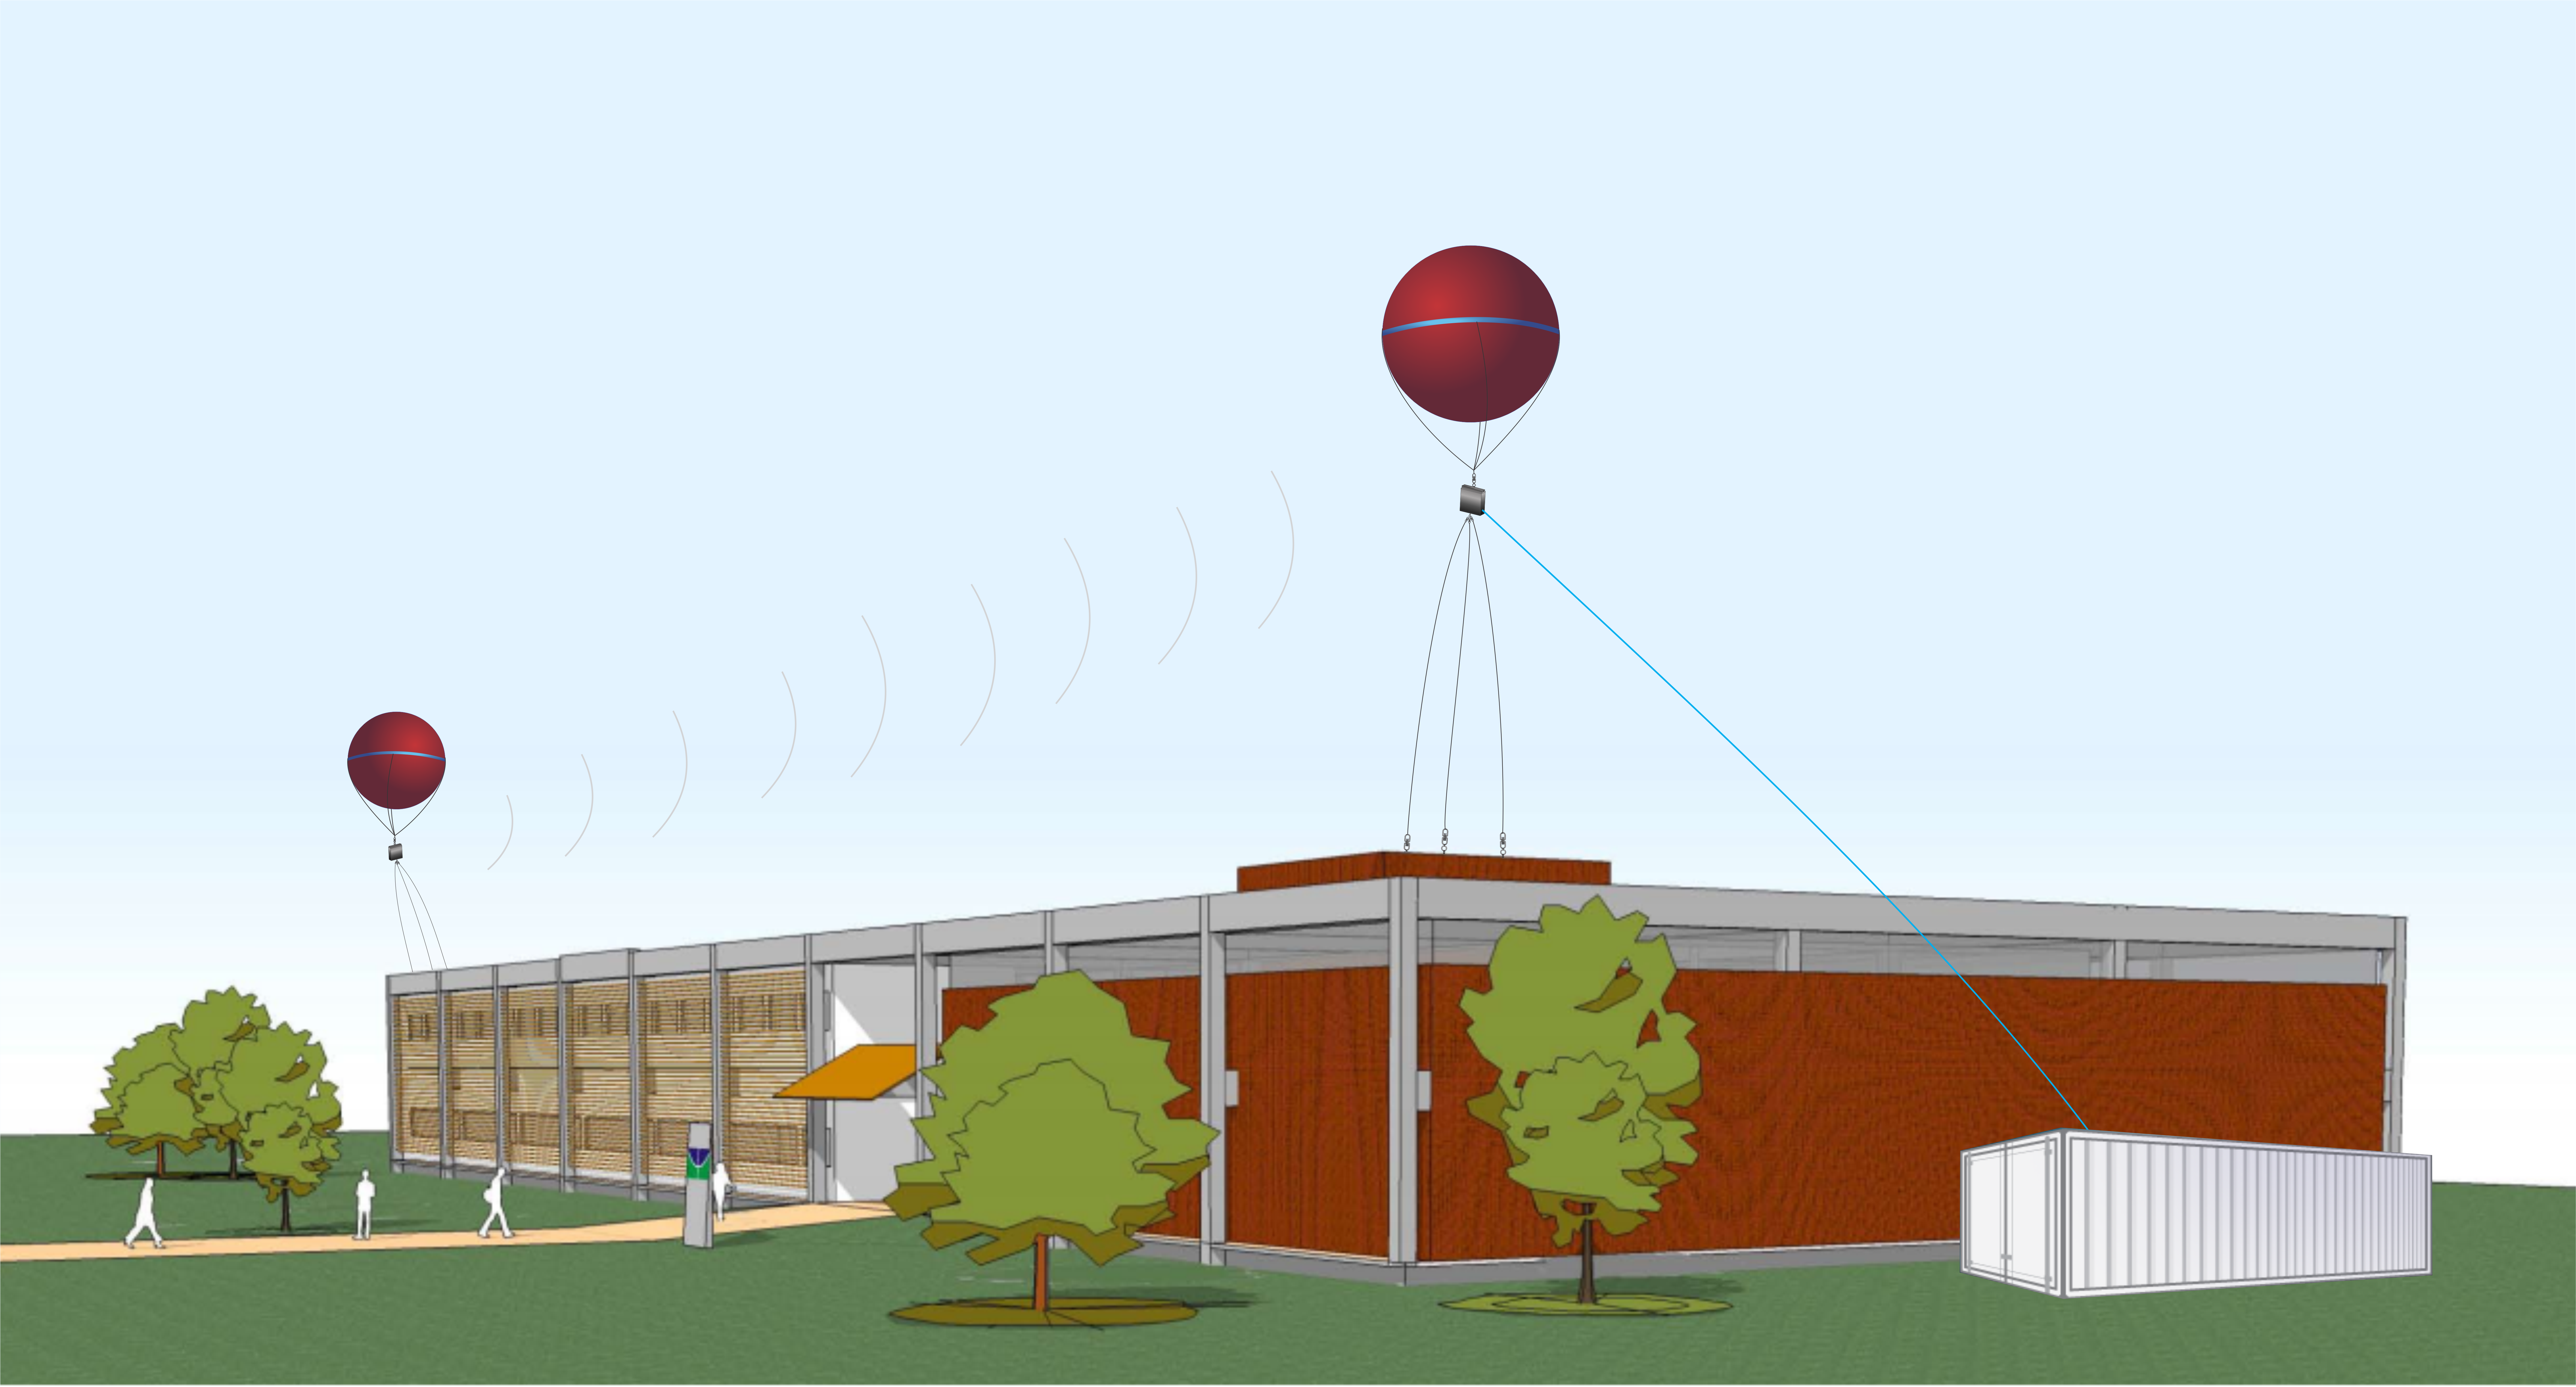
\includegraphics[width=\textwidth]{figuras/ilus-fun-sum}
\label{img:ilus-fun-sum}
\end{figure}

\begin{enumerate}

\item O balão cativo  SP (Super Pressão)  consistirá de uma bexiga (figura \ref{img:payload}), carga útil, cabeamento de sustentação (figura \ref{img:sustentacao}) e base de ancoramento.  Este necessitará de três pontos de fixação. Destes três, dois pontos estarão fixos no topo do respectivos prédios e o terceiro ponto será fixado em um poste de sustentação que terá a altura do prédio cerca de 10 metros de altura e estará distante 5 metros perpendicularmente ao mesmo.  A bexiga é o componente capaz de gerar uma sustentação, força que promove a subida do balão, e que será preenchida com um tipo de gás menos denso que o ar, gerando força para cima.

\begin{figure}[htp]
\centering
\caption{Protótipo da bexiga, \textit{payload} e cabos de sustentação feitos no software CATIA.}
\includegraphics[width=0.6\textwidth]{figuras/balaoRenderizado}
\label{img:payload}
\end{figure}

O gás do balão sairá do envelope a uma taxa baixa por semana, de acordo com as características do material do envelope, sendo necessária a reposição de gás a cada 4 meses. Para isso, serão instalados em dois pontos fixos dos prédios motores elétricos e será utilizado o cabo de aço Alma de Fibra.

O desenvolvimento da solução está disposto no Subprojeto de Estrutura e Sistema Aéreo, localizado na seção \ref{sec:subprojeto_de_estrutura_e_sistema_a_reo}.

\item A carga útil ou \textit{payload} (figura \ref{img:sustentacao}), é a unidade formada por uma estrutura portando todos  os equipamentos eletrônicos que promovem o monitoramento desejado. Por exemplo, câmeras, sensores, microcontroladores. Toda a transmissão de dados entre o balão e a estação de solo será feita por meio de ondas de rádio em uma faixa de frequências autorizada pelo órgão nacional competente , a ANATEL. Possuirá também um sistema de estabilização da carga para que as imagens possam ser transmitidas sem interferências.

\begin{figure}[htp]
\centering
\caption{Protótipo da \textit{payload} e cabos de sustentação feitos no software CATIA.}
\includegraphics[width=0.6\textwidth]{figuras/PAYLOADRENDERIZADA}
\label{img:sustentacao}
\end{figure}

O desenvolvimento da solução está disposto no Subprojeto de Eletrônica Embarcada, na seção \ref{sec:subprojeto_da_eletr_nica_embarcada}.

\item A estação de solo possui como função a recepção dos vídeos transmitidos pelo balão, de forma que um operador possa efetuar um diagnóstico do que acontece no estacionamento do campus. Tal estação deve ser capaz de estabelecer a recepção de vídeos de todos os balões do sistema SUM operantes na área de análise.

O sistema presente na estação de solo identifica se  está acontecendo alguma ação suspeita. Ao identificar,  aciona os operadores via rádio  para que eles verifiquem o motivo do alerta feito pela estação (figura \ref{img:processo}).

	\begin{figure}[H]
		\centering
		\caption{Processo 1- Funcionamento SUM. Fonte: Do autor, 2015.}
		\includegraphics[width=\textwidth]{figuras/processo}
		\label{img:processo}
	\end{figure}


	O desenvolvimento da solução está disposto no Subprojeto da Estação de Solo, na seção \ref{sec:subprojeto_da_esta_o_de_solo}.

\item O sistema de alimentação do SUM será OnGrid, ou seja, via rede de distribuição, e sistema de back up com 18 baterias estacionárias de 70 amperes dando 6 horas de autonomia.  O consumo do SUM será de 4712,35 kWh/mês. O desenvolvimento da solução está disposto no Consumo Energético, na seção \ref{sec:consumo_energ_tico}.

\end{enumerate}
